\chapter{alphazero\_baseline}
\label{chap:baseline}
\section{ニューラルネットワーク}
モデルの構成を図\ref{fig:baselineNetwork}に示す.
alphazero\_baselineにおける選択肢は列の数と等しい7であるため,1$\times$7の行列となる.
例えば方策が
$\left\{0, 0.1, 0.2, 0, 0, 0.7, 0.8\right\}$であるとき,方策中の最も大きい成分は7番目の0.8であるため,プレイヤーは次に7列目を選択する事が推奨される.
\begin{figure}[htbp]
	\centering
	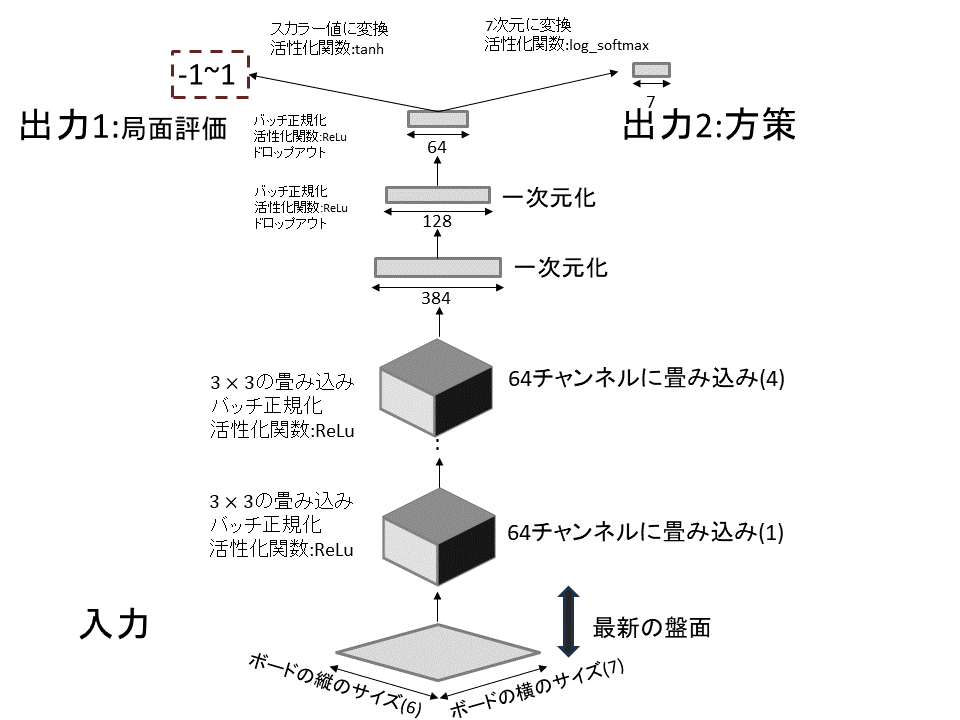
\includegraphics[width=\linewidth]{./figure/baselineNetwork.png}
	\caption{alphazero\_baselineネットワークの構成}
	\label{fig:baselineNetwork}
\end{figure}
また,モデルの訓練過程は以下のステップをまとめて1エポックとしたサイクルによって構成されている.
使用したテストデータ\cite{dataset}はα-β木探索によるconnect4の解から生成されている\cite{scoring}.
\begin{enumerate}
	\item 500ゲーム分の自己対戦を行う
	\item 自己対戦によって収集した盤面を入力としてネットワークを訓練
    \item ネットワークを教師データによって評価
    \item 新しいネットワークを用いたAIと訓練前の最善のネットワークを用いたAIによる対戦を50ゲーム分行い,6割以上
    の勝率を記録した場合,新しいネットワーク最善のネットワークとして保存する

\end{enumerate}
本論文の第3章におけるインタフェース実験で用いた「強いAI」のニューラルネットワークは上記をステップを200エポック分実行して訓練した場合の最善のモデルを使用している.

また,ネットワーク訓練時のパラメータの値を\ref{table:param-train}に示す.
\begin{table}[H]
	\caption{ネットワーク訓練時のパラメータ名と値}
	\centering
	\scalebox{0.98}[0.98]{
		\begin{tabular}{c|c}
			パラメータ名 & 値 \\ \hline
			学習率(lr)    & 0.001 \\ 
			dropout    & 0.3 \\
			epochs      & 5 \\
			batch\_size     & 64 \\
			num\_channels  & 64 \\
		\end{tabular}
	}
	\label{table:param-train}
\end{table}
\section{alphazero\_baselineのパラメータ更新}
alphazero\_baselineのパラメータ更新は第2章で述べた手順とほぼ同一であるが,$U(s, a)$の定義と$Q(s, a)$の更新則に差異がある.
($ C_{\textrm{cpuct}}$はハイパーパラメータ,$N(s), N(s, a)はそれぞれs,(s, a)に対して探索を行った回数$)
\begin{equation}
	{U(s, a)= C_{\textrm{cpuct}}P(s, a)\frac{\sqrt{N(s)}}{1+N(s, a)}\\
	}
\end{equation}

$Q(s, a)$は以下のように更新される.
($s_c = T(s, a_m), a_m = \underset{a}{argmax}{Q(s, a)+U(s, a)}$)
\begin{equation}
	{Q(s, a)=\frac{N(s, a)Q(s, a)+V(s_c)}{N(s, a)+1}\\
	}
\end{equation}
これらの変更を加えたalphazero\_baselineにおけるPV-MCTSアルゴリズムをAlgorithm\ref{alg:base}に示す.
\newpage

\begin{algorithm}
    \caption{PV-MCTS in alphazero-baseline (変更部分)}
    \label{alg:base}
    \begin{algorithmic}[1]
    \small
        \State $t$: 決定木
        \State $T$: 遷移関数
        \State $N(s, a)$: $(s, a)$の組み合わせを探索した回数
        \State $Q(s, a)$: 行動価値関数 ($\textrm{Explore}(s)$の平均)
        \State $W(s, a)$: 行動価値の総和$(W(s, a)=Q(s, a)N(s, a))$
        \State $P(s, a)(=P(s_n), s_n=T(s, a))$: 
        \State ニューラルネットワークから出力された方策
        \State $V(s, a)(=V(s_n), s_n=T(s, a))$: 
        \State ニューラルネットワークから出力された局面評価
        \Function{TreePolicy}{$s$}
            \If {$s$が探索されていない子ノードを持つとき}
                \State $s_c \gets T(s, a)$ ($s_c$は未探索のノード)
                \State \Call{InitNode}{$s_c$}
                \State \Return $a$
            \Else
                \State 各行動に対して$U(s, a)$を計算
                \State \underline{$U(s, a)= C_{\textrm{cpuct}}P(s, a)\frac{\sqrt{N(s)}}{1+N(s, a)}$}
                \State $(N(s)=\Sigma N(s, a))$
                \State 以下のように$a$を求める
                \State $a = {\underset{a}{\textrm{argmax}}} (Q(s, a)+U(s, a))$
                \State \Return $a$
                
            \EndIf
        \EndFunction
        \Function{Backpropagate}{$\zeta, G$}
            \For {each node-action pair $(s, a)$ in $\zeta$}
                \State $N(s, a) \gets 0$
                \State $W(s, a) \gets 0$
                \State $Q(s, a) \gets 0$
            \EndFor
        \EndFunction
        \Function{InitNode}{$s$}
            \For {each action $a$ from  $s$}
                \State $N(s, a) \gets N(s, a)+1$
                \State $W(s, a) \gets W(s, a)+G$
                \State \underline{$Q(s, a) \gets \frac{N(s, a)Q(s, a)+V(s_c)}{N(s, a)+1}$}
				\State $(s_c = T(s, a))$
            \EndFor
        \EndFunction
    \end{algorithmic}
\end{algorithm}